\section{Background} 

\subsection{Stair Climbing and Gaiting}  

Stair climbing is a non-linear task that engages multiple muscle groups and requires balancing the torso. Ascending stairs requires one leg to be fixed on the ground to maintain balance while the other leg swings through the trajectory trajectory\cite{hicks2012temporal}. Several studies have examined how people climb upstairs. Motion capture is one tool that can be used to record human kinematics and kinetics  \cite{chalodhorn2007learning} \cite{hu2014online} \cite{huang2018learning}. The work conducted in \cite{andriacchi1980study} and \cite{hicks2011lower} focused on the kinematics and dynamics of stair climbing by using a variety of motion capture, force plates, and IMUs sensors. These studies have produced high-resolution joint angle data for level ground walking and stair climbing.

\subsection{Learning from Demonstration}  

Learning from Demonstration (LfD) is the process of transferring skills to a robot by demonstration or example \cite{siciliano2016springer}\cite{Calinon2018} \cite{kormushev2011imitation} \cite{calinon2007teacher}. There are several steps in LfD: demonstration modality, motion primitives, and encoding methods. There are several steps in the LfD process, as stated below. 

\begin{enumerate} 
    \item Learning the demonstration 
    \item Recognition of the task 
    \item Encoding of the motion 
    \item Retrieval of the task 
    \item Reproduction of task 
\end{enumerate} 

The following two teaching modalities could be used to teach a  robot to follow a trajectory. The first teaching modality is kiniestic teaching; this modality involves a user moving a robot passively or running an impedance controller through a task while recording the joint positions of torques \cite{Calinon2018}. Researchers have applied kinetic teaching for upper limb robotic systems for industry and human-robot interfaces. While this method is a natural method of teaching, it is not well suited for teaching lower limb movement because it would require directly moving a leg through a gait motion. It would be difficult to replicate the leg's motion by the manual moving of a person or robot. 

The other teaching modality is visual observation. In this teaching modality, visual sensors record the desired motions and intentions of a demonstration for mapping onto a robotic system \cite{CalinonLee19}. In visual observation, motion capture systems (mocap) is the standard method. Marker system allows for precise tracking with millimeter accuracy of points on a person \cite{ott2008motion}. Due to is wide adaption and high accuracy for gait data collection\cite{ViconGaiting}, it is the method of data recording in this paper. There is a great deal of research on upper body control and very little research on lower body control based on motion control. This paper will show a method of using lower body mapping and recognition. 

Dynamic Motion Primitives (DMPS) are a method of breaking down demonstrations into their fundamental building blocks. Motion primitives aim to encode trajectories into building blocks that can then be rearranged and manipulated. DMP are a popular form of motion primitives \cite{ijspeert2013dynamical}. They work by creating a stable underline model and generating a forcing function to drive the system.  

In the classical formulation of DMPs, the model places radial basis functions (RBF) along the trajectory that pull the system towards the goal. DMPs are considered one of the gold standards of learning and replicating human motion \cite{nakanishi2004learning}. GMR provides a more comprehensive approach to the RBF placement and allows for the encoding of multiple trajectories, while DMP is limited to a single demonstration for training. 

There are several LfD methods for learning trajectories, including Gaussian Mixed Regression (GMR), Hidden Markov Models (HMM), and Locally Weighted Regression (LWR). They are all methods of encoding motion into basis functions for learning and reproduction. All the methods are similar but contain their pros and cons. LWR is the simplest method with GMR and HMM being extensions of this method, and therefore will not be considered.

In GMR, the demonstrations are encoded using Gaussian Mixture Models (GMM)\cite{calinon2013compliant} \cite{Statisticaldynamical}. The demonstration for training the model must be temporally scaled using Dynamic time warping (DTW).  GMR is computationally fast and produces smooth and continuous trajectories.  The benefits of using GMR are the following \cite{Calinon}: 

\begin{enumerate}  
    \item Allows encoding of local correlation between motion variables   
    \item Provides a principled approach to estimate the parameters of the radial base functions (RBF)  

    \item Reduce the number of RBF   
    \item Online estimation of the DMP parameters and model selection   
\end{enumerate}  

Hidden Markov Models (HMM) combines temporal scaling and transition probabilities through a double stochastic process \cite{calinon2007learning}. HMM offers several benefits over the GMR method. HMM has built-in temporal scaling, meaning that it can deal with demonstrations that are not aligned. However, the double stochastic process does not necessarily produce smooth and continuous trajectories. This property of HMM makes it not well suited for learning trajectories for exoskeletons.      

The proposed method presented in this paper is broken down into four steps; 1) collection of gait data, 2) encoding of motion into radial basis functions (RBF), 3) learning of regression function, 4) reproduction, and manipulation of the trajectories. \autoref{fig:demostation} illustrates the workflow for training and reproduction.

To collect the necessary data for reproduction, a motion capture trial was conducted, producing a set trajectory for learning. The trajectories were extracted and segmented. Using Gaussian Mixed Model (GMM), the trajectories were encoded into RBF, placed throughout the data set. The forcing function is found using Gaussian Mixed Regression (GMR), which regresses over the RBFs. This forcing function is then used to drive the Dynamic motion primitives (DMP), model. This procedure allows for manipulation for temporal, start, and goal manipulation.  
% \\  

% GMM probabilistically encodes the motion into Gaussian clusters distributed over the demonstration data. GMM is an extension of K-means; however, instead of a hard assignment of a point into a cluster, it is given a soft assignment  \cite{CalinonLee19}.  In other words, $K$-means a point is assigned either a $0$ or $1$ probability of belonging to a cluster. In contrast, in GMM, it is assigned a probability between $0$ and $1$. Expectation-Maximization algorithm does the assignment, which attempts to find the best placement of the points into the clusters. In doing so, it attempts to find the means and covariance of the clusters. The exit criteria of the iterative loop are the convergence of the log-likelihood.  



% The proposed method used motion capture data to record demonstrations, GMM to encode the demonstrations into radial basis functions (RBFs). This  RBFs are placed throughout the training data set. GMR then regresses the RBFs to find a forcing function that drives the model from the start to the goal. DMP for playback and manipulation of the trajectory. The start, goal, and time can all be changed at run time. \autoref{fig:demostation} illustrates the workflow for training and reproduction. 

  

\begin{figure} 
    \centering 
    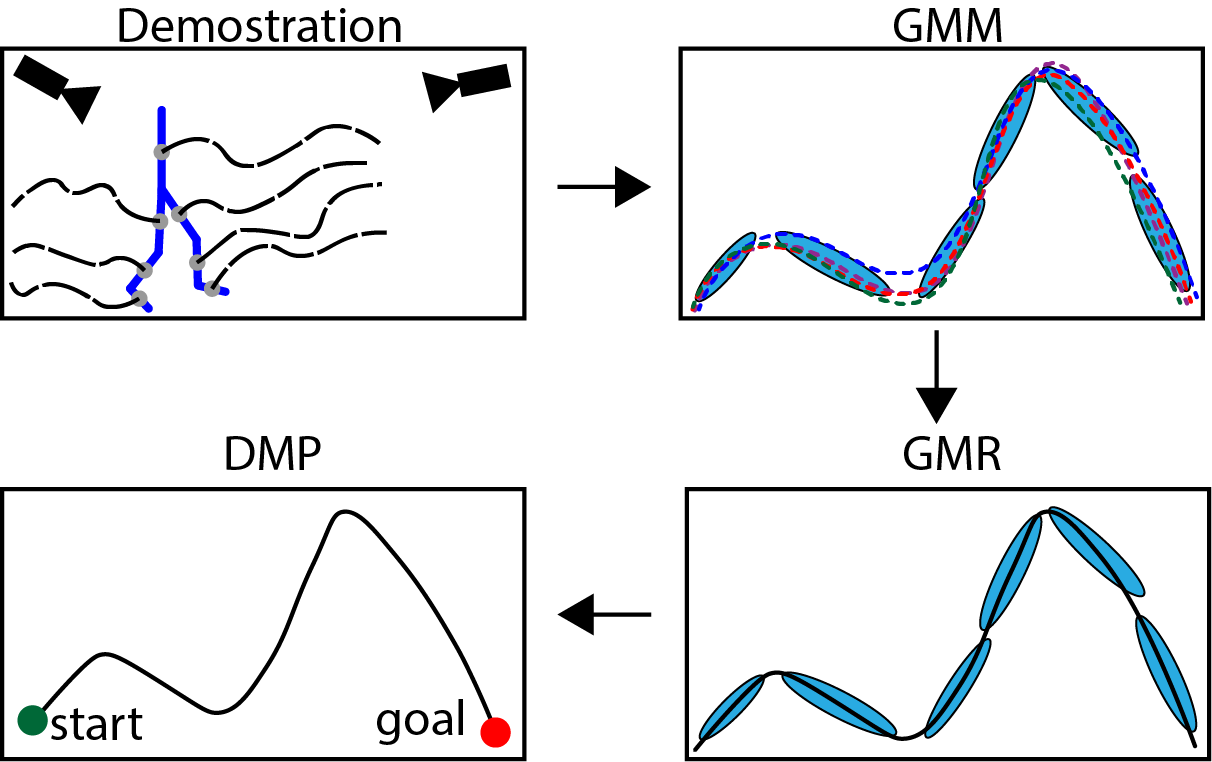
\includegraphics[scale=0.8]{images/demostation.png} 
    \caption{Order of operations of the learning. The First step is to collect and extract the motion data. The raw data is then encoded using GMM. The motion is then extracted using GMR. Finally the motion is replicated using DMPs } 
    \label{fig:demostation} 
\end{figure} 